\subsection{Impact Simulation Results}

The coupled ODE system was integrated over a five-year horizon ($t \in [0, 1825]$~days)
using an explicit Runge--Kutta solver (RK45, $\Delta t_{\max} = 1$~day) for two scenarios:
a \emph{baseline} with no active intervention ($u(t)=0$, $\Lambda_{\text{opt}}=0$, $\Delta\beta=0$)
and an \emph{optimized} scenario whose parameters are derived from the surveillance
optimization output (\S\ref{sec:optimization}): fire suppression
$u_{\text{opt}} = 0.513$,
enforcement boost $\Lambda_{\text{opt}} = 3.110$,
and tourism mortality reduction $\Delta\beta = 15%$.

Table~\ref{tab:impact-populations} compares final populations after five years.
Every species benefits from the optimized resource allocation, with lions showing
the largest relative improvement ($+72.4\%$)
and black rhino recovering above their initial count in the optimized scenario.

\begin{table}[H]
\centering
\caption{Final populations after five years under baseline and optimized scenarios.}
\label{tab:impact-populations}
\begin{tabular}{lrrr}
\hline
\textbf{Species} & \textbf{Baseline} & \textbf{Optimized} & \textbf{Change} \\
\hline
    Plains zebra & 8,277 & 9,080 & +9.7\% \\
    Lion & 218 & 377 & +72.4\% \\
    Elephant & 1,683 & 2,248 & +33.6\% \\
    Black rhino & 52 & 80 & +55.9\% \\
\hline
\end{tabular}
\end{table}

Table~\ref{tab:impact-deaths} summarises cumulative mortality averted by the intervention.

\begin{table}[H]
\centering
\caption{Cumulative deaths over five years and deaths averted by the optimized strategy.}
\label{tab:impact-deaths}
\begin{tabular}{lrrrr}
\hline
\textbf{Species} & \textbf{Baseline} & \textbf{Optimized} & \textbf{Averted} & \textbf{Averted \%} \\
\hline
    Plains zebra & 2,699 & 2,022 & 677 & 25.1\% \\
    Lion & 498 & 345 & 154 & 30.9\% \\
    Elephant & 1,404 & 908 & 497 & 35.4\% \\
    Black rhino & 62 & 42 & 20 & 31.8\% \\
\hline
\end{tabular}
\end{table}

\begin{figure}[H]
\centering

\includegraphics[width=\textwidth]{impact_population_trajectories.png}
\caption{Population trajectories for four keystone species under baseline (dashed red)
and optimized (solid blue) scenarios.  Shaded regions indicate the population gain
attributable to the surveillance and intervention strategy.}
\label{fig:impact-pop}
\end{figure}

\begin{figure}[H]
\centering

\includegraphics[width=\textwidth]{impact_threat_dynamics.png}
\caption{Threat dynamics over the five-year simulation.  Wildfire intensity $F(t)$ shows
seasonal peaks during the dry season (day~180 of each year); the optimized scenario
suppresses fire more effectively.  Poaching effort $P(t)$ declines under increased
enforcement.  Tourism disturbance $T(t)$ is identical between scenarios (exogenous driver)
but its mortality impact is reduced by the waterhole dispersion interventions.}
\label{fig:impact-threats}
\end{figure}

\begin{figure}[H]
\centering
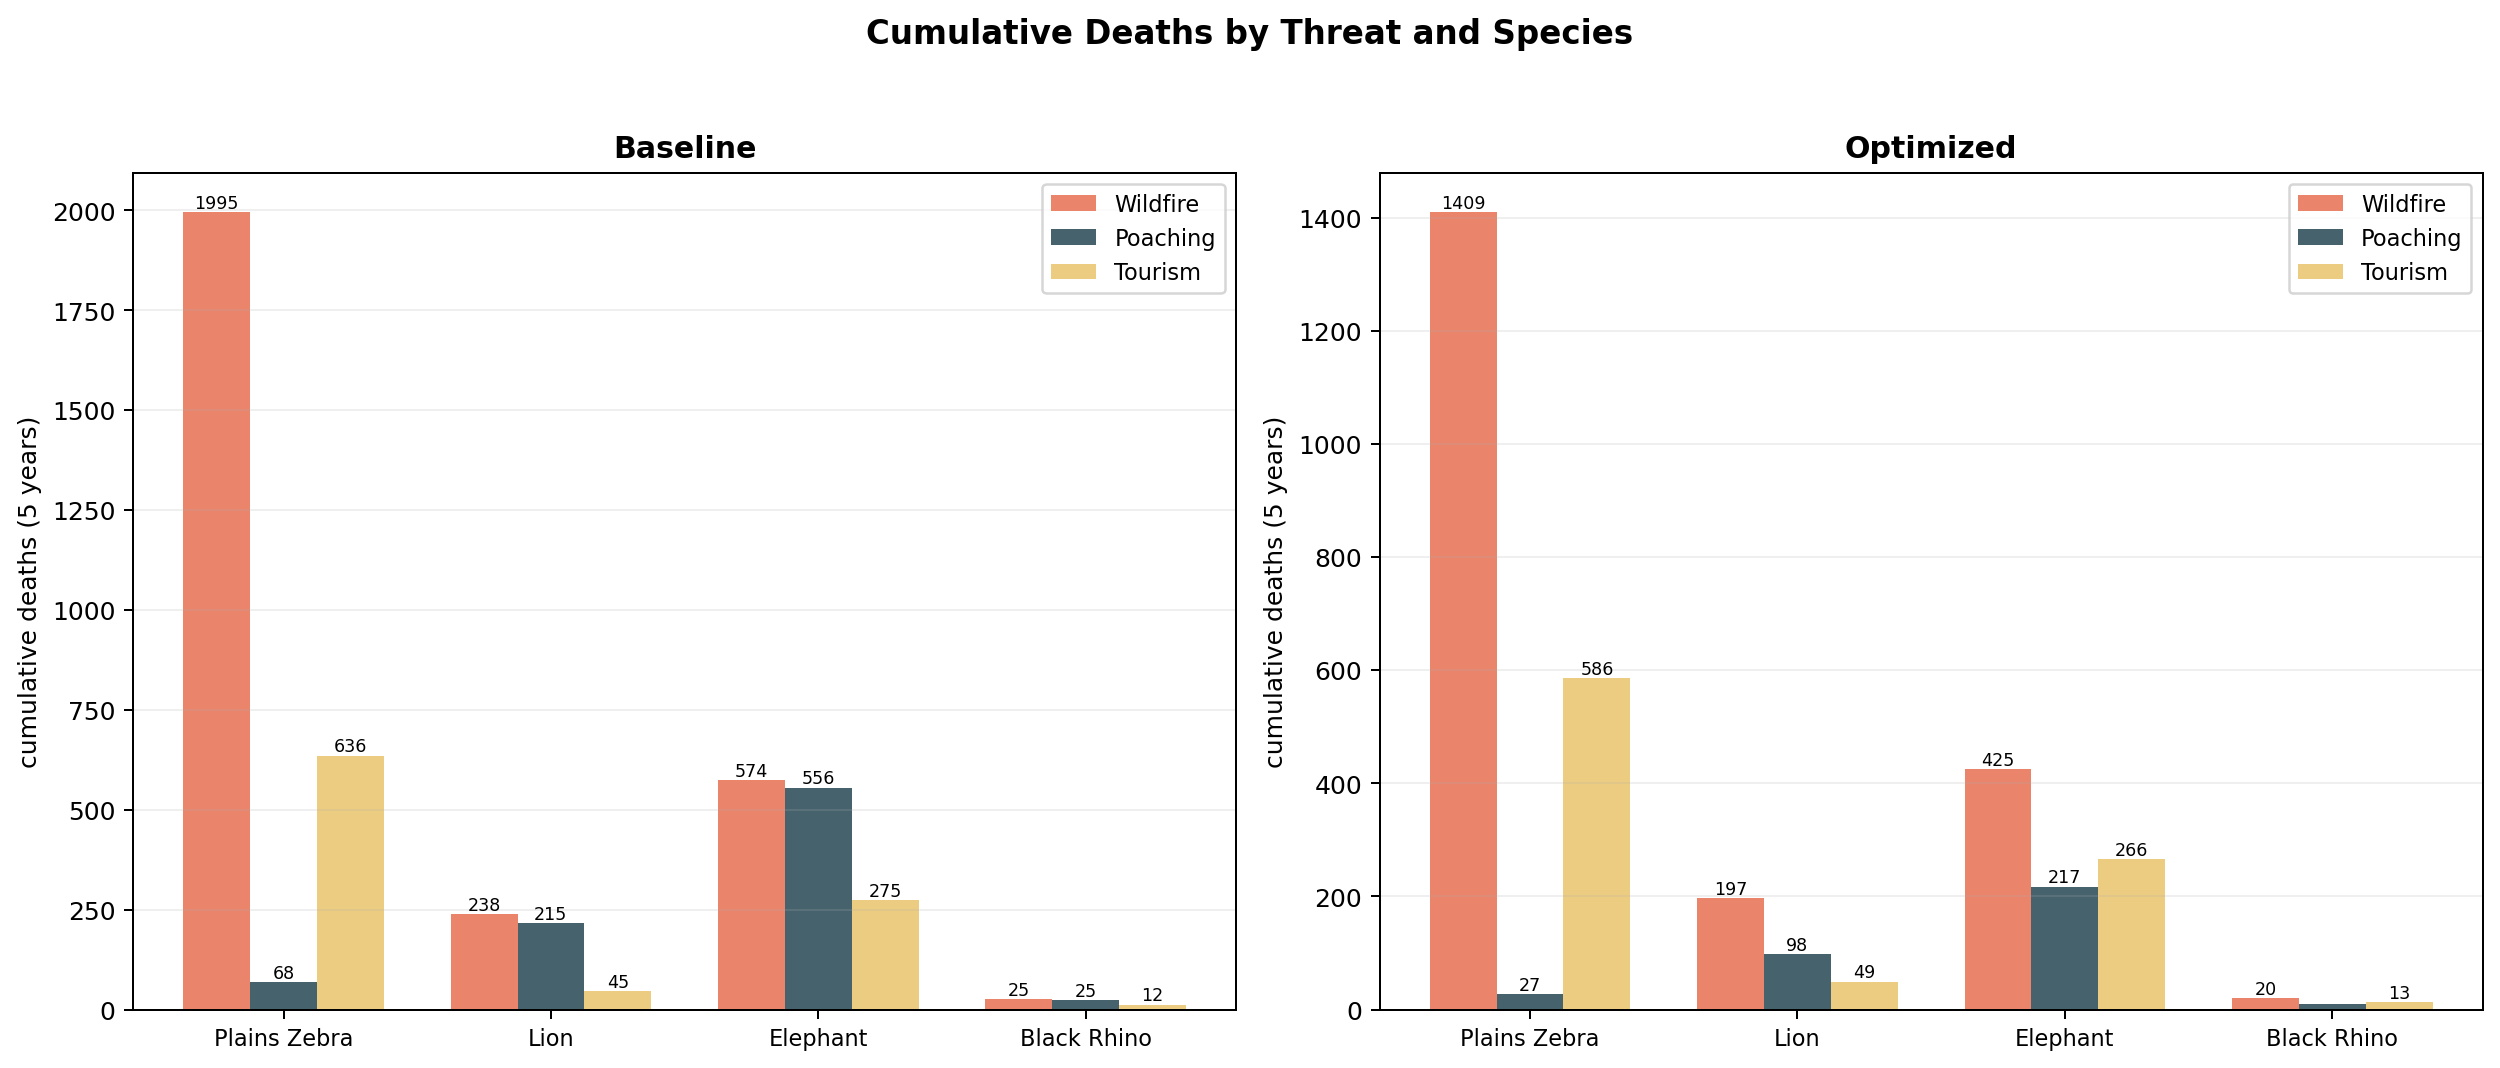
\includegraphics[width=\textwidth]{impact_cumulative_deaths.png}
\caption{Cumulative deaths over five years disaggregated by threat type.  Wildfire is the
dominant source of mortality for all species; the optimized scenario reduces fire-related
deaths through faster suppression response.}
\label{fig:impact-deaths}
\end{figure}

\begin{figure}[H]
\centering

\includegraphics[width=\textwidth]{impact_carrying_capacity.png}
\caption{Resource dynamics (top) and resulting carrying capacities (bottom).
Fire and tourism degrade water, forage, and space; carrying capacity $K_s(t)$
is set by the most limiting resource via Liebig's law.  Dotted lines show
actual populations $N_s(t)$ for comparison.}
\label{fig:impact-capacity}
\end{figure}
